
\appendix

\chapter{Cartographer configuration} \label{app:cartographer}
\pagenumbering{Roman} 				
\setcounter{page}{1}

The following configuration file was used during the real-world experiments:

\begin{lstlisting}
include "map_builder.lua"
include "trajectory_builder.lua"

options = {
  map_builder = MAP_BUILDER,
  trajectory_builder = TRAJECTORY_BUILDER,
  map_frame = "map",
  tracking_frame = "imu_link",
  published_frame = "base_link",
  odom_frame = "odom",
  provide_odom_frame = false,
  publish_frame_projected_to_2d = false,
  use_odometry = true,
  use_nav_sat = false,
  use_landmarks = false,
  num_laser_scans = 1,
  num_multi_echo_laser_scans = 0,
  num_subdivisions_per_laser_scan = 1,
  num_point_clouds = 0,
  lookup_transform_timeout_sec = 0.2,
  submap_publish_period_sec = 0.3,
  pose_publish_period_sec = 5e-3,
  trajectory_publish_period_sec = 30e-3,
  rangefinder_sampling_ratio = 1.,
  odometry_sampling_ratio = 1.,
  fixed_frame_pose_sampling_ratio = 1.,
  imu_sampling_ratio = 1.,
  landmarks_sampling_ratio = 1.,
}

MAP_BUILDER.use_trajectory_builder_2d = true
MAP_BUILDER.num_background_threads = 7

TRAJECTORY_BUILDER_2D.num_accumulated_range_data = 1
TRAJECTORY_BUILDER_2D.min_range = 0.5
TRAJECTORY_BUILDER_2D.max_range = 24.95
TRAJECTORY_BUILDER_2D.min_z = -1
TRAJECTORY_BUILDER_2D.max_z = 2.
TRAJECTORY_BUILDER_2D.use_imu_data = true
TRAJECTORY_BUILDER_2D.ceres_scan_matcher.translation_weight = 5
TRAJECTORY_BUILDER_2D.ceres_scan_matcher.rotation_weight = 7
TRAJECTORY_BUILDER_2D.missing_data_ray_length = 5
TRAJECTORY_BUILDER_2D.use_online_correlative_scan_matching = false
TRAJECTORY_BUILDER_2D.submaps.grid_options_2d.resolution = 0.20
TRAJECTORY_BUILDER_2D.submaps.num_range_data = 25

POSE_GRAPH.optimize_every_n_nodes = 15

POSE_GRAPH.optimization_problem.local_slam_pose_translation_weight = 1e6
POSE_GRAPH.optimization_problem.local_slam_pose_rotation_weight = 1e4
POSE_GRAPH.optimization_problem.odometry_translation_weight = 1e4
POSE_GRAPH.optimization_problem.odometry_rotation_weight = 1e7

return options
\end{lstlisting}

\chapter{Source code}

All implementations are written in C++ for ROS Melodic and provided in the electronic attachment. They are also available on the author's GitHub page: \url{https://github.com/jhlenes/complete_coverage} and \url{https://github.com/jhlenes/usv_simulator}. 

\section{Complete coverage maneuvering system}

The complete coverage maneuvering system contains the following ROS packages:

\begin{itemize}

\item \textbf{\path{coverage_binn}:} Implementations of BINN CCPP and circular cell partitioning.

\item \textbf{\path{coverage_boustrophedon}:} Implementations of boustrophedon motions CCPP and square cell partitioning. Also contains the simple Dubins path implementation.

\item\textbf{\path{guidance}:} Implementation of the LOS guidance law.

\item \textbf{\path{map_inflating}:} Configuration of map inflation.

\item \textbf{\path{mr_obs_connector}:} Implementation of the interface to Maritime Robotics' onboard system.

\item\textbf{\path{nmea_navsat_driver}:} Implementation of the slightly modified GNSS driver.

\item\textbf{\path{otter_slam}:} Configuration of Cartographer SLAM.

\item\textbf{\path{sensors}:} Configuration of drivers for lidar, IMU and GNSS. Also contains the configuration for the EKF.

\item\textbf{\path{usv_msgs}:} Definition of a message format that contains speed and course values.

\end{itemize}

\section{Simulator}

The simulator contains the following ROS packages:

\begin{itemize}

\item \textbf{\path{otter_control}:} Implementations of thrust allocation and controllers for speed and course control.

\item \textbf{\path{otter_description}:} Description of the Otter USV, including location of thrusters and a 3D model for visualization.

\item \textbf{\path{otter_gazebo}:} Configuration of simulated sensors, thrusters and dynamics.

\item \textbf{\path{usv_gazebo_plugins}:} Implementation of the simulator copied from \citet{website:vrx}.

\item \textbf{\path{usv_worlds}:} Description of simulation environment with locations of obstacles.

\end{itemize}

\section{Running the code}

After installing the packages in ROS Melodic, the system can be run by following these steps. The commands must be typed into a separate terminal. \\

\noindent If the system is running on the actual Otter USV, this step can be skipped. Otherwise, simulate the Otter USV with:
\begin{lstlisting}[language=bash]
roslaunch otter_gazebo otter.launch
\end{lstlisting}

\noindent \\ If the system is running on the simulated Otter USV, start this guidance:
\begin{lstlisting}[language=bash]
roslaunch guidance sim_guidance.launch
\end{lstlisting}
\noindent Otherwise, if the system is running on the actual Otter USV, start this guidance:
\begin{lstlisting}[language=bash]
roslaunch guidance real_guidance.launch
\end{lstlisting}

\noindent \\ Start the boustrophedon motions complete coverage path planning with:
\begin{lstlisting}[language=bash]
roslaunch coverage_boustrophedon coverage.launch
\end{lstlisting}
\noindent Alternatively, start the bio-inspired neural network complete coverage path planning with:
\begin{lstlisting}[language=bash]
roslaunch coverage_binn coverage_binn.launch
\end{lstlisting}

\section{Playing back logged data}

ROS bagfiles are included in the electronic attachment and can be played back to visualize the experiments. \\

\noindent Start the visualization with:
\begin{lstlisting}[language=bash]
roslaunch coverage_boustrophedon visualize.launch
\end{lstlisting}

\noindent \\ Play back the selected log file with:
\begin{lstlisting}[language=bash]
rosbag play filename.bag
\end{lstlisting}



\chapter{Video from the first experiment}

A video demonstrating the first experiment is included in the attachment and also available at \url{https://youtu.be/hqOUKtosnFw}. The video shows both the the Otter USV's behavior in the water, and the complete coverage maneuvering system's visualization, see \figref{fig:video}.

\begin{figure}[h!]
	\centering
	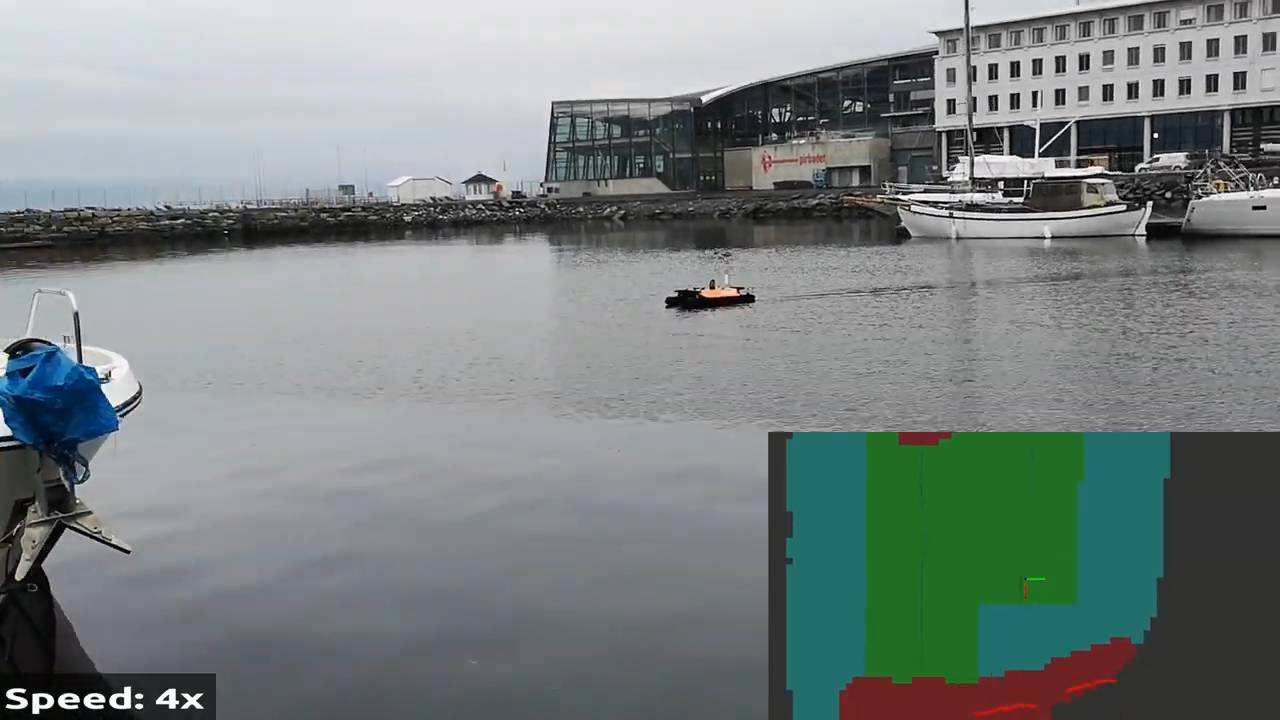
\includegraphics[width=1\textwidth]{fig/video.jpg}
	\caption{Screenshot of video.}
	\label{fig:video}
\end{figure}


